\documentclass{article}
\usepackage{graphicx}
\usepackage{hyperref}
\usepackage[utf8]{inputenc}
\usepackage{enumerate}
\begin{document}
\pagenumbering{gobble}
\begin{center}
    \rule{0pt}{0pt}
    \vfill
    
\includegraphics[scale=0.9]{logo.png}\\
    {\huge Software Requirements Specification\\}
    for project\\
    {\Large Semantic Pipelines Editor\\}
    by\\
    {\large\href{mailto:kelpeart@fel.cvut.cz}{Artem Kelpe}, \href{mailto:dorosyan@fel.cvut.cz}{Yan Doroshenko}\\}
    \vfill
    \rule{0pt}{90pt}\\
    {\large Czech Technical University in Prague\\} \today
\end{center}
\newpage
\tableofcontents
\newpage
\pagenumbering{arabic}
\setcounter{page}{3}
\section{Introduction}
\subsection{Purpose}
This document describes the Semantic Pipelines Editor software, a specialized graph editor for the Semantic Pipelines framework, as of version 1.0.
\subsection{Intended Audience}
This document is intended for developers, interested in Semantic Pipelines Editor, Semantic Pipelines infrastructure and its integration structure.
\subsection{References}
\href{http://json-ld.org/primer/latest/}{JSON-LD Primer}\\
\href{https://www.w3.org/TR/rdf11-primer/}{RDF Primer}\\
\href{http://ieeexplore.ieee.org/document/6011704/?arnumber=6011704\&tag=1}{\textit{P. Křemen, Z. Kouba}, Ontology-Driven Information System Design}\\
\href{http://2016.eswc-conferences.org/sites/default/files/papers/Accepted\%20Posters\%20and\%20Demos/ESWC2016\_DEMO\_JOPA.pdf}{ESWC 2016, JOPA: Efficient Ontology-based Information System Design}
\section{Overall Description}
\subsection{Product Scope}
Semantic Pipelines Editor is an application, whose purpose is to be integrated with Semantic Pipelines framework and to provide a graphical editor in form of an oriented graph for it with a possibility to execute pipelines from the editor itself. It is also capable of module saving and loading, which is provided by persisting data into the ontology storage. The main goal is to provide a free and open source software edition tool for the above-stated framework and to enable developers to interact and manage pipelines in a self-explanatory and convenient way without having to deal with proprietary software or restrictive licenses.
\subsection{Product Functions}
Product functions can be divided into two groups:
\begin{itemize}
    \item Graph CRUD operations
    \item Pipeline execution
\end{itemize}
Functions are described in more detail in chapter \hyperref[sec:features]{System Features}.
\subsection{User Classes and Characteristics}
Users are distinguished based on user rights, specified in the ontology storage. As of version 1.0 rights are the following:
\begin{enumerate}
    \item Create pipelines\\
	User having this right can create new pipelines.\\
	Applicable FRQs:\\
	FRQ1,FRQ2
    \item Load pipelines\\
	This right allows user to load pipelines from ontology storage.
	Applicable FRQs:\\
	FRQ1,FRQ3
    \item Save pipelines\\
	This right provides possibility to save pipelines into ontology storage.
	Applicable FRQs:\\
	FRQ1,FRQ4
    \item Alter pipelines\\
	User granted this right is allowed to add/remove nodes and edges to the pipeline.
	Applicable FRQs:\\
	FRQ1,FRQ5
    \item Execute pipelines\\
	This right lets user to execute pipelines.
	Applicable FRQs:\\
	FRQ1,FRQ6,FRQ7,FRQ8,FRQ9
    \item See execution history\\
	User having this right can see the history of pipeline execution.
	Applicable FRQs:\\
	FRQ1,FRQ10
    \item Debug modules\\
	User can execute modules in debug mode only if he has this right.
	Applicable FRQs:\\
	FRQ1,FRQ11
    \item User management\\
	User having this right is allowed to add/remove other user's rights.
	Applicable FRQs:\\
	FRQ1,FRQ12
\end{enumerate}
Each user can be granted any or none of this rights.
\subsection{Operating Environment}
Operating environment consists of several parts:
\begin{itemize}
    \item Application Server\\
	The software is meant to be run inside of a container like an application server. Originally Semantic Pipelines Editor was designed to run inside of Tomcat 8 application server, but should work in any other.
    \item Database Server\\
	The application is designed to work with RDF4J ontology storage.
    \item Semantic Forms\\
	Functionality is partially dependent on the Semantic Forms to be available as a web service.
\end{itemize}
\subsection{Design and Implementation Constraints}
There are several constraints that rigidly specify the product's relation to the infrastructure and possible ways of application.
\begin{itemize}
    \item Semantic Forms Integration\\
	Semantic Pipelines Editor is relying on Semantic Forms for the form generation so the WS communication is done in a very specific way which requires bigger changes for the form generation strategy to be replaced.
    \item Ontology Storage\\
	Data is stored in the ontology storage (RDF4J), which makes for the specific way of entity objects design.\\
	Another constraint regarding ontology is a very limited set of frameworks and libraries available, which also influences the implementation.
    \item Java/Scala Interoperability\\
	All the business logic of the application is implemented in Scala programming language. This is done in order to minimize the unnecessary (from the business standpoint) implementation details for the logic layer to be clearer and more refined for the developer. However, Scala's interoperability with Java is limited in some specific areas.\\
    \item JavaScript-based client
	Semantic Pipelines Editor has a thin client and most of user interaction is made with JavaScript. Therefore the application is meant to be accessed with a web browser that is can run JavaScript code.
\end{itemize}
\subsection{Third Party Dependencies}
\begin{itemize}
    \item JDK
	Oracle JDK or OpenJDK is required for running the backend
    \item Scala SDK
	Scala SDK is required for running the backend
    \item Spring
	Several components of the Spring Framework are used for IoC
    \item JOPA
	Persistence layer is done with JOPA
    \item Apache Maven
	Apache Maven build tool is used for building the project and sources generation
    \item JUnit
	Testing is partially made with JUnit
    \item ServletAPI
	ServletAPI is required by the web application 
    \item Logback
	Logback is used for logging
    \item JSON-Core
	JSON-Core is required for JSON operations in Java and Scala
    \item Jaxb-JSONLD-Jackson
	Jaxb-JSON-LD-Jackson provides JSON-LD support
    \item Mockito
	REST WS testing is done with Mockito
    \item Sigma.js
	Sigma.js is providing frontend graph representation
    \item ReactJS
	ReactJS is required for UI implementation
\end{itemize}
\section{External Interface Requirements}
\subsection{User Interfaces}
Interaction with the user is provided by a web interface, built around the JavaScript library for graph representation Sigma.js. The main window consists of two parts: left panel and a working surface for editing graphs (\hyperref[pic1]{Figure 2}). Left panel contains elements for authorization, saving and loading graph and list of available types of nodes that can be added to the graph. Search feature with autocompletion provides more convenient navigation. At the working surface user can see the current graph (loaded or created), edit it (move nodes, draw edges etc.). Node double click shows the form generated from this node and its dependencies in the popup (\hyperref[pic2]{Figure 3}). User management is done in the separate window (\hyperref[pic3]{Figure 4}).
\subsection{Software Interfaces}
Application consists of frontend and backend parts with backend accessing the ontology storage as well as a Semantic Pipelines web service. Communication between backend and frontend is implemented with JSON-LD format messages sent through REST API. All communication is done through unsecured HTTP protocol. Authentication encryption is provided by integrated Spring Security tools. 
\section{System Features}
\subsection{Functional Requirements}
\label{sec:features}
\begin{enumerate}[FRQ1]
    \item \textbf{See pipelines}\\
	Pipelines are represented in form of an oriented graph. Nodes represent modules and edges are dependencies between them, which makes for intuitive and functional user interface.
    \item \textbf{Create pipelines}\\
	There exists a possibility for creating new pipelines from scratch by adding individual modules and dependencies between them.
    \item \textbf{Load pipelines}\\
	The software allows loading pipelines from the ontology storage.
    \item \textbf{Save pipelines}\\
	The software allows saving pipelines into the ontology storage.
    \item \textbf{Alter pipelines}\\
	Pipelines can be modified by adding or deleting modules, changing their properties and dependencies between them.
    \item \textbf{Execute pipeline to point}\\
	Certain module of a pipeline can be executed. During execution module dependencies are processed recursively.
    \item \textbf{Execute entire pipeline}\\
	Execution of the entire pipeline can be done. In this case all the modules are executed.
    \item \textbf{See execution progress}\\
	Semantic Pipelines Editor provides user with an indication of execution progress.
    \item \textbf{See execution results}\\
	The results are shown once execution is finished.
    \item \textbf{See execution history}\\
	There is a possibility to see the history of executions of a pipeline.
    \item \textbf{Module debug}\\
	Modules can be executed with debug flags.
    \item \textbf{Manage users}\\
	Users granted special permission can manage other user's access to the application's features.
\end{enumerate}
\subsection{System Limitations}
As of version 1.0 the application does not feature the following capabilities:
\begin{itemize}
    \item Creating new module types
    \item Editing module type definitions
    \item Communication with other systems in a format different from JSON-LD
    \item Serving as a general-purpose graph editor
\end{itemize}
	\section{Other Requirements}
	\begin{itemize}
	    \item The application is licensed under the \href{https://www.gnu.org/licenses/gpl.txt}{GNU GPLv3} license
	\end{itemize}
	\section*{Appendix A: Diagrams}
	\addcontentsline{toc}{section}{Appendix A: Diagrams}
	\begin{figure}[h!]
	    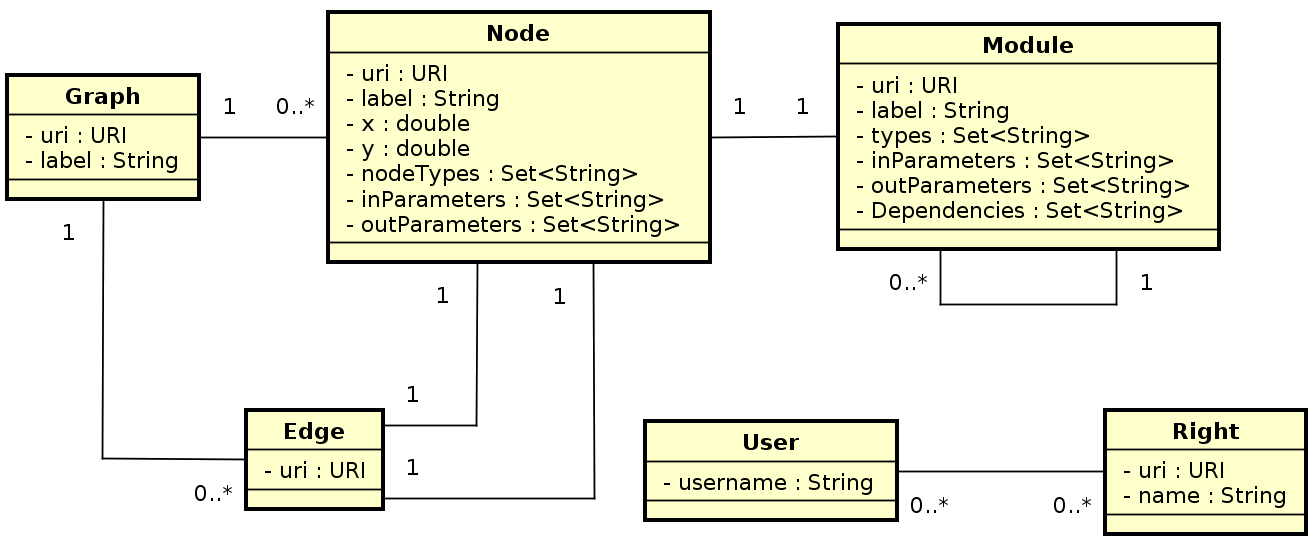
\includegraphics[width=\textwidth]{ClassDiagram.png}
	    \caption{Class Diagram}
	\end{figure}
	\section*{Appendix B: Glossary}
	\addcontentsline{toc}{section}{Appendix B: Glossary}
	\textbf{API} - Application Programming Interface\\
	\textbf{FRQ} - Functional requirement\\
	\textbf{JDK} - Java Development Kit\\
	\textbf{JOPA} - Java OWL Persistence API\\
	\textbf{JSON} - JavaScript Object Notation\\
	\textbf{JSON-LD} - JavaScript Object Notation for Linked Data\\
	\textbf{OWL} - Web Ontology Language\\
	\textbf{RDF} - Resource Description Framework\\
	\textbf{RDF4J} - RDF for Java programming language\\
	\textbf{REST} - Representational State Transfer\\
	\textbf{SDK} - Software Development Kit\\
	\textbf{UI} - User Interface\\
	\textbf{WS} - Web service
	\newpage
	\section*{Appendix C: Illustrations}
	\addcontentsline{toc}{section}{Appendix C: Illustrations}
	\begin{figure}[h!]
	    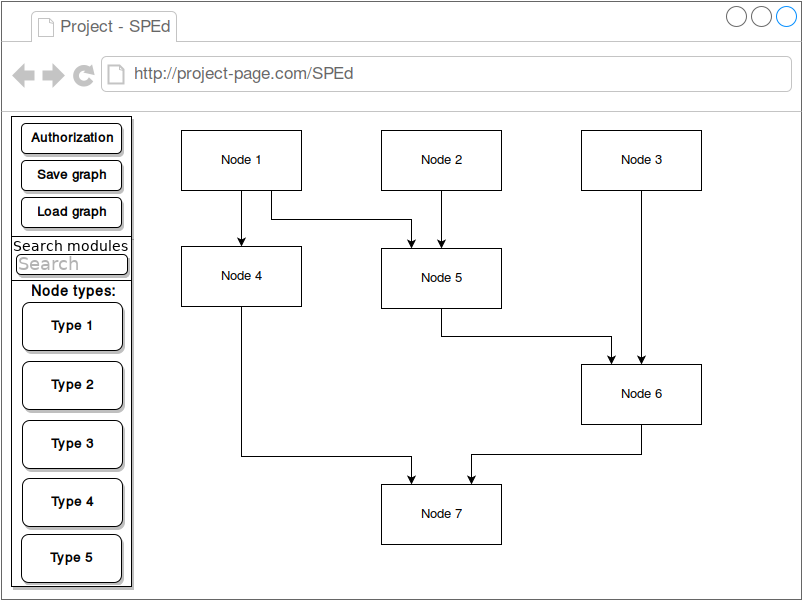
\includegraphics[width=\textwidth]{pic1.png}
	    \label{pic1}
	    \caption{Main window}
	\end{figure}
	\begin{figure}[h!]
	    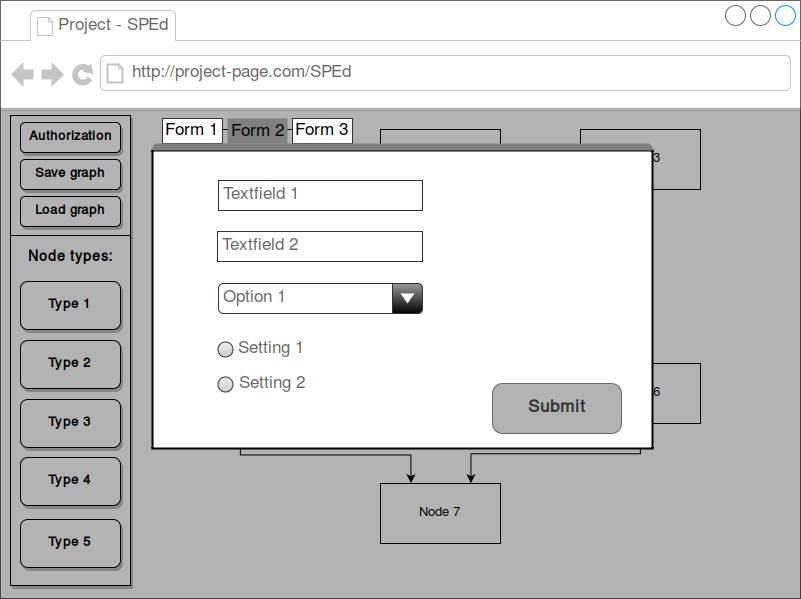
\includegraphics[width=\textwidth]{pic2.png}
	    \label{pic2}
	    \caption{Generated form}
	\end{figure}
	\begin{figure}[h!]
	    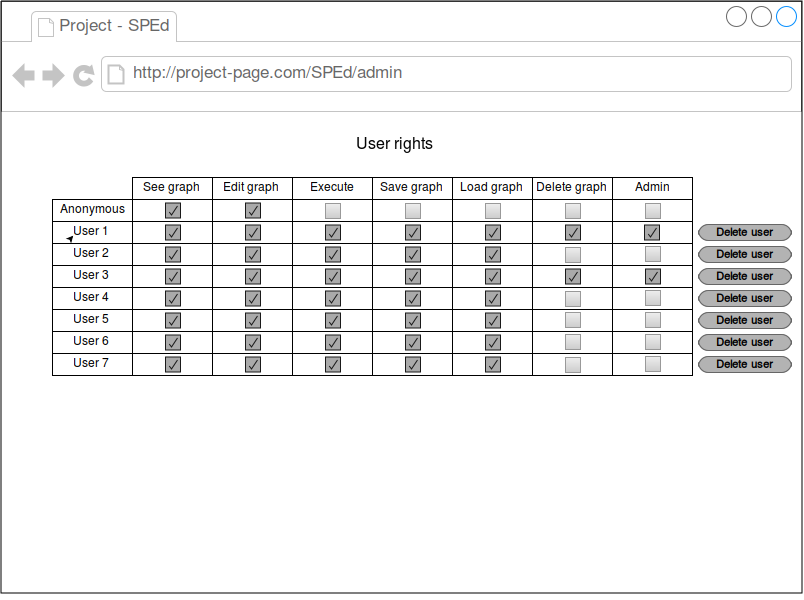
\includegraphics[width=\textwidth]{pic3.png}
	    \label{pic3}
	    \caption{User management window}
	\end{figure}
\end{document}
